\documentclass[10pt,a4paper]{article}
\usepackage[utf8]{inputenc}
\usepackage[english]{babel}
\usepackage{amsmath}
\usepackage{amsfonts}
\usepackage{amssymb}
\usepackage{graphicx}
\usepackage{bm}
\usepackage{xspace}
\usepackage[left=2cm,right=2cm,top=2cm,bottom=2cm]{geometry}
\setcounter{MaxMatrixCols}{20}
\usepackage[capitalise]{cleveref}
\usepackage[per-mode=symbol]{siunitx}
\usepackage{url}

\newcommand{\xk}{\ensuremath{\bm{x}_k}\xspace}
\newcommand{\yk}{\ensuremath{\bm{y}_k}\xspace}
\newcommand{\xkk}{\ensuremath{\bm{x}_{k+1}}\xspace}
\newcommand{\xx}[1]{\ensuremath{\bm{x}_{#1}}\xspace}
\newcommand{\uk}{\ensuremath{\bm{u}_k}\xspace}
\newcommand{\ukk}{\ensuremath{\bm{u}_{k+1}}\xspace}
\newcommand{\uu}[1]{\ensuremath{\bm{u}_{#1}}\xspace}
\newcommand{\duk}{\ensuremath{\bm{\dot{u}}_k}\xspace}
\newcommand{\dukk}{\ensuremath{\bm{\dot{u}}_{k+1}}\xspace}
\newcommand{\duu}[1]{\ensuremath{\bm{\dot{u}}_{#1}}\xspace}
\newcommand{\ek}{\ensuremath{\bm{e}_k}\xspace}
\newcommand{\ekk}{\ensuremath{\bm{e}_{k+1}}\xspace}
\newcommand{\ee}[1]{\ensuremath{\bm{e}_{#1}}\xspace}
\newcommand{\rk}{\ensuremath{\bm{r}_k}\xspace}
\newcommand{\ymin}{\ensuremath{\bm{y}_\text{min}}\xspace}
\newcommand{\ymax}{\ensuremath{\bm{y}_\text{max}}\xspace}
\newcommand{\umin}{\ensuremath{\bm{u}_\text{min}}\xspace}
\newcommand{\umax}{\ensuremath{\bm{u}_\text{max}}\xspace}
\newcommand{\dumin}{\ensuremath{\bm{\dot{u}}_\text{min}}\xspace}
\newcommand{\dumax}{\ensuremath{\bm{\dot{u}}_\text{max}}\xspace}
\newcommand{\epsy}{\ensuremath{\epsilon_{y}}\xspace}
\newcommand{\epsu}{\ensuremath{\epsilon_{u}}\xspace}
\newcommand{\epsdu}{\ensuremath{\epsilon_{\dot{u}}}\xspace}
\newcommand{\epst}{\ensuremath{\epsilon_T}\xspace}
\newcommand{\code}[1]{\texttt{#1}\xspace}
\newcommand{\R}{\ensuremath{\mathbb{R}\xspace}}
\newcommand{\ts}{\ensuremath{t_s}}
\newcommand{\Co}{\ensuremath{C_1}}
\newcommand{\Cc}{\ensuremath{C_2}}
\def\pwidth{0.49}

\begin{document}

\section{Problem formulation}

The \code{MPCProblem} class permits to solve Model Predictive Control (MPC) problems.
The class considers the following state space representation of the system
\begin{align}
    \xkk &= A\xk + B\uk\\
    \yk &= \Co\xk
\end{align}
where $\xk \in \R^n$, $\yk \in \R^q$, and $\uk \in \R^p$ represent the state of the system, the output, and the control at time step $k$, respectively.
$A \in \R^{n \times n}$, $B \in \R^{n \times p}$, and $\Co \in \R^{q \times n}$ are the state, the control, and the output matrices.
The matrices given to the class are the discrete time matrices, so if you have the continuous time state space representation of your system, you should first discretize it for a particular sampling time.

In general, the \code{MPCProblem} class solves the following quadratic optimization problem over the time horizon $T$:
\begin{equation}
    \label{eq:min}
    \min_s s^\intercal Q s
\end{equation}
with
\begin{equation}
    \label{eq:s}
    s = [\bm{e}, \bm{u}, \bm{\dot{u}}, \epsy, \epsy, \epsdu, \epst]
\end{equation}
subject to
\begin{align}
    \uu{0} &= \bm{u}^* \label{eq:u0}\\
    \ek &= \Co\xk - \rk,\quad k = 0,\dots,T \label{eq:error}\\
    -\epst &\leq \ee{T} \leq \epst \label{eq:terminal}\\
    \ukk &= \uk + \duk \cdot \ts,\quad k = 0,\dots,T-1 \label{eq:duk}\\
    \Cc\xkk &\leq \ymax + \epsy,\quad k = 0,\dots,T-1 \label{eq:ymax}\\
    \Cc\xkk &\geq \ymin - \epsy,\quad k = 0,\dots,T-1 \label{eq:ymin}\\
    \ukk &\leq \umax + \epsu,\quad k = 0,\dots,T-1 \label{eq:umax}\\
    \ukk &\geq \umin - \epsu,\quad k = 0,\dots,T-1 \label{eq:umin}\\
    \ukk - \uk &\leq \dumax\cdot\ts + \epsdu,\quad k = 0,\dots,T-1 \label{eq:dumax}\\
    \ukk - \uk &\geq \dumin\cdot\ts - \epsdu,\quad k = 0,\dots,T-1 \label{eq:dumin}\\
    \epsy &\geq 0 \label{eq:epsy}\\
    \epsu &\geq 0 \label{eq:epsu}\\
    \epsdu &\geq 0 \label{eq:epsdu}\\
    \epst &\geq 0 \label{eq:epst}\\
\end{align}
where
\begin{equation}
    \label{eq:xk}
    \xk = A^{k} \xx{0} + \sum_{i=0}^{k-1} A^{k-i-1}B \uu{i}
\end{equation}

In \cref{eq:min}, $s$ is the minimization variable and $Q$ a diagonal matrix, which can be modified by the user to weight the minimization terms.
The $Q$ matrix must be positive definite, so all entries on the diagonal must be strictly positive.
This is required because of the resolution method used by the solver, which requires problems to be strictly convex.
This kind of problem is simpler to solve, so the solution can be computed very efficiently.
In turn, we cannot set diagonal entries to 0, which requires the problem to be expressed in a non-intuitive way.
For example, in standard MPC problems \xk is part of the state so, for example, the error constraint is formulated as
\begin{align}
    \xkk &= A\xk + B\uk\\
    \ek &= \Co\xk - \rk,
\end{align}
which is much easier to read than the combination of \cref{eq:error,eq:xk}.
Clearly, \xk should not be part of the minimization: you want to minimize the error, not the state.
With a solver accepting semi-definite programs, this is not a problem, as we can simply set the diagonal entries of the $Q$ matrix regarding the \xk terms to 0.
With the QuadProg++\footnote{\url{https://github.com/liuq/QuadProgpp}} solver used in here this is not possible, and this is the reason why the problem is formulated in a more ``complex'' way.

The $s$ variable is composed by a set of subvariables:
\begin{itemize}
    \item $\bm{e}$, output error: this is the set of output errors for each time step $k$ in the considered time horizon. $\ek \in \R^q$ is the difference between the output of the system ($\Co\xk$) and the target reference value ($\rk$) (constraint in \cref{eq:error}) for $k = 0,\dots,T$.
    \item $\bm{u}$, control: this is the set of control actions for each time step $k$ in the considered time horizon, with $\uk \in \R^p$ for $k = 0,\dots,T-1$. The first value (\uu{0}) is fixed and it is a parameter of the problem (\cref{eq:u0}).
    \item $\bm{\dot{u}}$, control derivative: this is the set of control derivatives, i.e., $\duk \in \R^q$ is the difference between \ukk and \uk (constraint in \cref{eq:duk}) for $k = 0,\dots,T-1$. This term is optional can can be disabled when instantiating the problem, disregarding the control derivative when minimizing.
    \item \epsy: slack variable for the violation of output constraints. This is optional and can be disabled when instantiating the problem. This removes the slack variable from the optimization problem and allows no constraint violation.
    \item \epsu: slack variable for the violation of control constraints. This is optional and can be disabled when instantiating the problem. This removes the slack variable from the optimization problem and allows no constraint violation.
    \item \epsdu: slack variable for the violation of control derivative constraints. This is optional and can be disabled when instantiating the problem. This removes the slack variable from the optimization problem and allows no constraint violation.
	\item \epst: slack variable for the terminal constraint. This is optional and can be disabled when instantiating the problem. This removes the slack variable from the optimization problem and transforms the terminal constraint into $\ee{T} = 0$.
\end{itemize}

With respect to the constraints, the interpretation is the following:
\begin{itemize}
    \item \cref{eq:terminal}: this is called the terminal constraint and indicates that, at the end of the time horizon, we want our output error to be zero, or very close to it. Notice that this might make the problem unfeasible, e.g., when setting a very small time horizon. For this reason, the constraint can be disabled. Alternatively to disabling the constraint, it is possible to enable a slack variable for it, so that the constraint can be violated but at a certain cost.
    \item \cref{eq:duk}: this constraint simply defines that two successive control actions differ by the control derivative. When the minimization on the control derivative is disabled, this constraint is not used.
    \item \cref{eq:ymax,eq:ymin}: constraints on output limiting the maximum and the minimum output value. Notice that we use a different output matrix than the one of the error constraint (\cref{eq:error}), which we call \Cc. The reason is simple: imagine that our state is composed by the acceleration and the speed of a vehicle and that we want to reach a target speed while limiting the acceleration. If we use the same output matrix this is not possible (if not with some ugly hack), but by using two different output matrices we increase the flexibility while lowering the computational effort. In the document and in the code, $\Cc \in \R^{q_2 \times n}$. These constraints can be violated if the slack variable for the output is enabled. If the slack variable on output is not enabled, then the \epsy variable is not considered.
    \item \cref{eq:umax,eq:umin}: constraints on control limiting the maximum and the minimum control value. These constraints can be violated if the slack variable for the control is enabled. If the slack variable on control is not enabled, then the \epsu variable is not considered.
    \item \cref{eq:dumax,eq:dumin}: constraints on control derivative limiting the maximum and the minimum control derivative value. The limit is multiplied by the sampling time \ts, so changing the sampling time doesn't require the user to change the \dumax and the \dumin values. These constraints can be violated if the slack variable for the control derivative is enabled. If the slack variable on control derivative is not enabled, then the \epsu variable is not considered.
    \item \cref{eq:epsy,eq:epsu,eq:epsdu,eq:epst}: these constraints simply force the slack variables to be positive.
\end{itemize}

Finally, \cref{eq:xk} defines \xk in terms of the variables of the problem.
\xx{0} and \uu{0} are the initial state and control action, respectively, while \uk for $k = 1,\dots,k-1$ are the control actions computed by the algorithm.

\section{Sample problem}

The library comes with a sample program (\texttt{test-mpc.cc}) that solves an MPC problem where the state is described by the following system of differential equations:
\begin{equation}
    \dot{\bm{x}} = \begin{cases}
        \dot{a} = -\frac{1}{\tau} a + \frac{1}{\tau} u\\
        \dot{v} = a
    \end{cases}
\end{equation}
The system state represents the acceleration and the speed of a vehicle, where the acceleration is subject to an actuation lag modeled as a first order lag with a time constant $\tau$.
By writing the system in the standard state-space representation we obtain
\begin{align}
    \dot{\bm{x}} &= G\bm{x} + H\bm{u}\\
    \bm{y} &= \Co\bm{x}
\end{align}
where
\begin{equation}
    G = \begin{bmatrix}-\frac{1}{\tau} & 0\\1 & 0\end{bmatrix},\quad H = \begin{bmatrix}\frac{1}{\tau}\\0\end{bmatrix},\quad \Co = \begin{bmatrix}0 & 1\end{bmatrix}
\end{equation}
We discretize the continuous time representation by transforming $H$ and $G$ into $A$ and $B$, respectively, so that the state-space representation now becomes
\begin{align}
    \xkk &= A\xk + B\uk\\
    \yk &= \Co\xk
\end{align}
where
\begin{equation}
    A = e^{G \cdot \ts},\quad B = \int_0^{\ts} e^{G \lambda} d\lambda H
\end{equation}
obtaining
\begin{equation}
    A = \begin{bmatrix}
        e^{-\frac{\ts}{\tau}} & 0\\
        \tau\left(1 - e^{-\frac{\ts}{\tau}}\right) & 1\\
    \end{bmatrix},\quad
    B = \begin{bmatrix}
        1 - e^{-\frac{\ts}{\tau}}\\
        \ts + \tau\left(e^{-\frac{\ts}{\tau}} - 1\right)
    \end{bmatrix}
\end{equation}
$A$, $B$, and $C$ are thus the matrices we pass to the \texttt{MPCProblem} class given a particular choice of the time constant $\tau$ and the sampling time \ts.

In the provided example, we set $\ts = \SI{0.1}{\second}$ and $\tau = \SI{0.5}{\second}$, obtaining
\begin{equation}
    A = \begin{bmatrix}
        0.8187 & 0\\
        0.09063 & 1\\
    \end{bmatrix},\quad
    B = \begin{bmatrix}
        0.1812\\
        0.009365\\
    \end{bmatrix}
\end{equation}
The initial state $\xx{0}$ and the initial control $\uu{0}$ are set to $[0, 0]^\intercal$ and $[0]$, respectively, the reference $\rk$ to $[1]$, the time horizon $T$ to 60 steps (\SI{6}{\second}), the terminal constraint is enabled, and there is no bound for output, control, and control derivative variables.
Finally all the weights in the $Q$ matrix are set to 1.

In the root folder you find a bash script (\texttt{test-mpc.sh}) that runs the test application under different output parameters.
If the scripts finds an \texttt{R} installation, it will also plot the results to some PDF files.

The first example (\cref{fig:test01}) shows the results for the default parameters, i.e., the ones previously described.
The graph shows the different quantities considered in the optimization problem, i.e., the actual speed and the target speed, the acceleration, the control input, and the control derivative.
As expected, the solution brings the system to the target speed minimizing also the effort on control and control derivative.

\begin{figure}[h]
    \centering
    \begin{minipage}[t]{\pwidth\textwidth}
        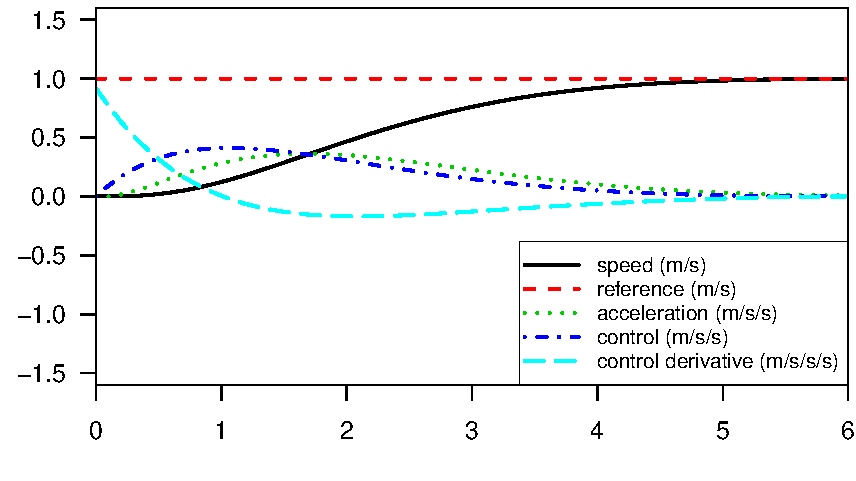
\includegraphics[width=\textwidth]{./fig/test01}
        \caption{Results for default parameters.}
        \label{fig:test01}
    \end{minipage}
    \hfill
    \begin{minipage}[t]{\pwidth\textwidth}
        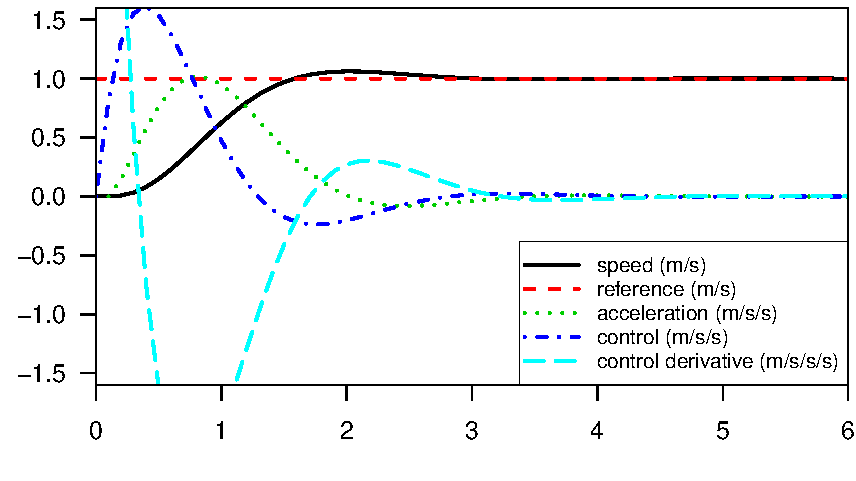
\includegraphics[width=\textwidth]{./fig/test02}
        \caption{Results for lower weights on control and control derivative.}
        \label{fig:test02}
    \end{minipage}
\end{figure}

In the second example (\cref{fig:test02}) we lower the weights for the control and the control derivative terms in the minimization, setting them to $0.01$ instead of $1$.
Control and control derivative are now much larger, as we told our solver that we do not care too much about minimizing them.
This results in a faster settling time.

In the third example (\cref{fig:test03}) we use the parameters of the second but we add upper and lower bounds on control actions, i.e., \SI{1}{\meter\per\second\squared} and \SI{-1}{\meter\per\second\squared}, respectively.
The result is very similar to the second, with the only difference that the control action is ``truncated'' at \SI{1}{\meter\per\second\squared} as per constraint.
This causes a slightly larger settling time with respect to the second example.

\begin{figure}[h]
    \centering
    \begin{minipage}[t]{\pwidth\textwidth}
        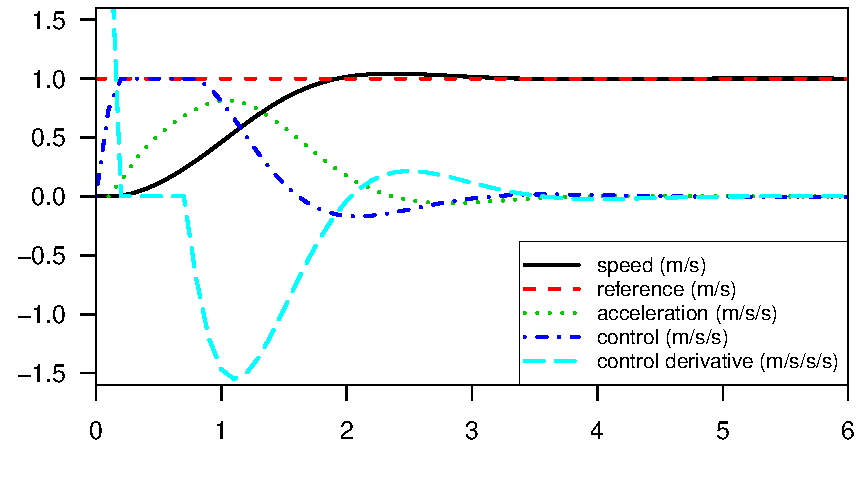
\includegraphics[width=\textwidth]{./fig/test03}
        \caption{Results for lower weights on control and control derivative, plus bounded control action.}
        \label{fig:test03}
    \end{minipage}
    \hfill
    \begin{minipage}[t]{\pwidth\textwidth}
        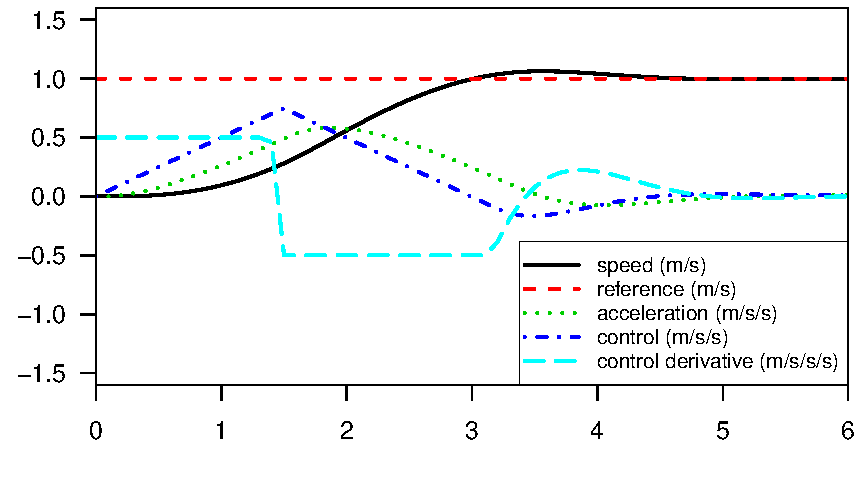
\includegraphics[width=\textwidth]{./fig/test04}
        \caption{Results for lower weights on control and control derivative, plus bounded control and control derivative action.}
        \label{fig:test04}
    \end{minipage}
\end{figure}

In the fourth example (\cref{fig:test04}), w.r.t. the third, we add a constraint on the control derivative as well, i.e., $\SI{-0.5}{\meter\per\second\cubed} \leq \duk \leq \SI{0.5}{\meter\per\second\cubed}$.
The result is pretty evident, both in terms of control derivative bounds and in terms of control input.
The bound on control derivative causes a ``linear'' increase and decrease of the control action.
The additional bound causes the settling time to increase.

The fifth example (\cref{fig:test05}) is the same as the second (i.e., we lower the weights for control and control derivative) but, in addition, we add a bound to the maximum acceleration (\SI{0.6}{\meter\per\second\squared}).
The plot shows that the system reaches the target speed, but the acceleration never exceeds the bound set by the constraint.

\begin{figure}[h]
    \centering
    \begin{minipage}[t]{\pwidth\textwidth}
        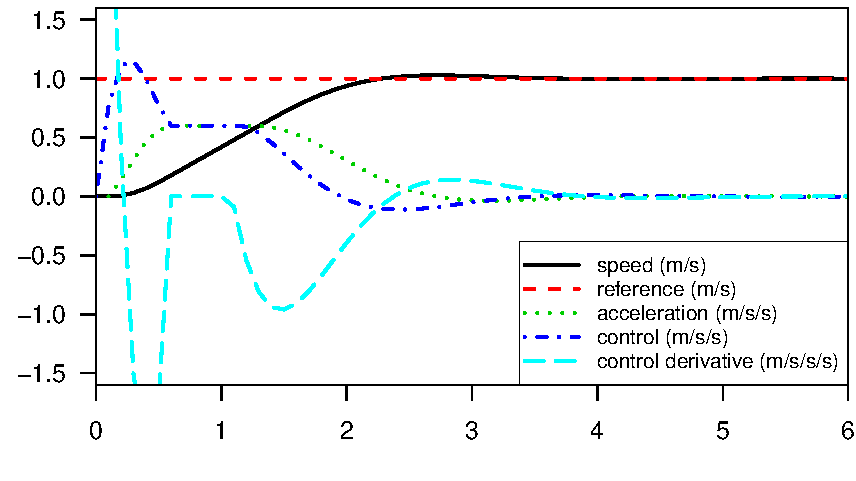
\includegraphics[width=\textwidth]{./fig/test05}
        \caption{Results for lower weights on control and control derivative, plus bound on acceleration.}
        \label{fig:test05}
    \end{minipage}
    \hfill
    \begin{minipage}[t]{\pwidth\textwidth}
        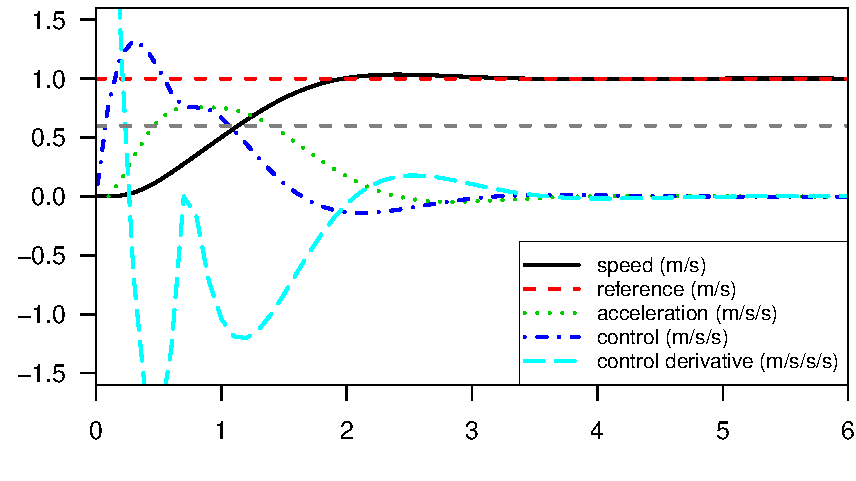
\includegraphics[width=\textwidth]{./fig/test06}
        \caption{Results for lower weights on control and control derivative, plus bound on acceleration and slack variable for output bounds enabled.}
        \label{fig:test06}
    \end{minipage}
\end{figure}

The final example (\cref{fig:test06}) enables the slack variable for the output constraint set in the fifth example, setting the weight penalization for the slack variable in the $Q$ matrix to 10.
In this case the solver is allowed to violate the constraint on acceleration, as it can bee seen in the plot.
The constraint bound is highlighted by the gray dashed line, and the solver exceeds this limit reaching roughly \SI{0.75}{\meter\per\second\squared}.

\end{document}
